\subsection{Анализ цепи с помощью метода узловых потенциалов(контурных токов)}


\subsubsection{Метод контурных токов}

При расчете данным методом полагаю, что в каждом независимом контуре течет свой контурный ток. Т.о. в данном методе за искомые принимаются контурные токи.

Систему уравнений приводим к следующему виду:



$$
\begin{cases}
R_{11} I_{11} + R_{12} I_{22}   = E_{11} \\
R_{21} I_{11} + R_{22} I_{22}   = E_{22} \\
\end{cases}
$$

В матричной форме:

\begin{equation}
[R][I]=[E]
\end{equation}
, где

$$
[R]=
\left[
\begin{array}{cc}
R_{11} & R_{12} \\
R_{21} & R_{22} 
\end{array}
\right]
$$

$$
[E]=
\left[
\begin{array}{cc}
E_{11} \\
E_{22} 
\end{array}
\right]
$$

$$
[I]=
\left[
\begin{array}{cc}
I_{11} \\
I_{22} 
\end{array}
\right]
$$

Уравнение решается методом Крамера:

\begin{equation}
I_{i} = \frac{\Delta_{i}}{\Delta}
\end{equation}

\subsubsection{Метод узловых потенциалов}

метод расчета электрических цепей путём записи системы линейных алгебраических уравнений, в которой неизвестными являются потенциалы в узлах цепи. В результате применения метода определяются потенциалы во всех узлах цепи, а также, при необходимости, токи во всех ветвях.

\begin{center}
	\begin{figure}[h!]
		\center{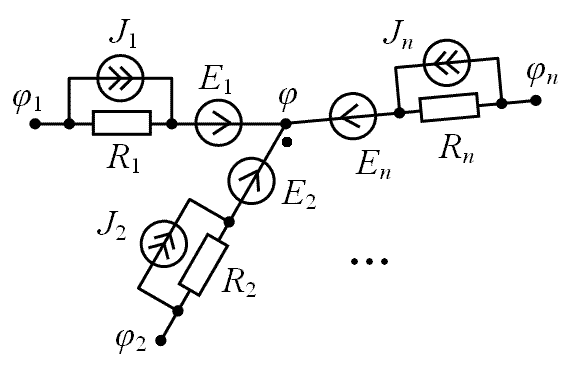
\includegraphics[scale=0.5]{usl_poteltional.png}}
		\caption{Схема}	
	\end{figure}
\end{center}	

По первому закону Кирхгофа для узла:

\begin{equation}
\sum_{i=1}^n I_i=0
\end{equation}

\begin{equation}
I_i = \frac{\phi_i - \phi + E_i}{R_i} + J_i
\end{equation}



\begin{equation}
\sum_{i=1}^n (\frac{\phi_i - \phi + E_i}{R_i} + J_i) = 0
\end{equation}

Составляем систему уравнений для n-1 узлов.



\pagebreak